%---------------------导言区---------------------------%
\documentclass[12pt,a4paper,UTF8]{ctexart}
	%10pt：正文字体为12pt，缺省为10pt；各层级字体大小会根据正文字体自动调整
	%a4paper：纸张大小a4；
	%UTF8：中文要求
\usepackage{geometry}%用于设置上下左右页边距
	\geometry{left=2.5cm,right=2.5cm,top=3.2cm,bottom=2.8cm}
\usepackage{xeCJK}
\usepackage{amsmath}
\usepackage{paralist}
\usepackage{enumerate}
\usepackage{booktabs}
\usepackage{multirow}
\usepackage{graphicx}
\usepackage{subfig}
\usepackage{setspace}
\usepackage{listings}
\usepackage{lastpage}
\usepackage{hyperref}
\usepackage{pdfpages}

%xeCJK：中文字体（如楷体，作者和机构需要用到）的设置
	%amsmath：数学公式
	%paralist，enumerate：自定义项目符号
	%booktabs：三线图，论文常用的表格风格
	%multirow：复杂表格
	%graphicx，float: 插入图片
	%subfig：并排排版图片、竖向排版图片
	%setspace：设置行间距等功能
	\setlength{\parindent}{2em}%正文首行缩进两个汉字
	%listings:用于排版各种代码；比如matlab的代码
	\lstset{language=Matlab}%matlab代码
	%lastpage:获取总页数;
	%hyperref:超链接,和lastpage搭配.
\usepackage{fancyhdr}
	%fancyhdr：一个很强大的宏包，用于自定义设计页面风格并命名以供调用。
	\pagestyle{fancy}
	\rhead{光泵磁共振实验}
	\lhead{近代物理实验~~~实验报告}
	\cfoot{Page \thepage/\pageref{LastPage}}  %当前页\总页数
	\rfoot{\today}
		%分别是右页眉、左页眉、中页脚、右页脚
	\renewcommand{\headrulewidth}{0.4pt}
	\renewcommand{\theenumi}{(\arabic{enumi})}

%%%%%%%%%%%%%%%%%%%%%%%%%%%%%%%%%%%%%%%%%%%%%%%%%%%%%%%%%%
%%%%%%%%%%%%%%%%%%%%%%%%%正文开始%%%%%%%%%%%%%%%%%%%%%%%%%%
%%%%%%%%%%%%%%%%%%%%%%%%%%%%%%%%%%%%%%%%%%%%%%%%%%%%%%%%%%

\graphicspath{{pics/}}
\begin{document}

%%begin-------------------标题与信息-----------------------%%

%%标题
\begin{center}
\LARGE\textbf{光泵磁共振实验}
\end{center}

%%信息
\begin{doublespacing}
	%doublespacing：手动两倍行距
	\begin{tabular}{lr}
	 & \\
	 {实验人姓名：徐殊行~23343071} & {合作者姓名：王志超~23343062}\\
	 {实验时间：2025年5月9日} & {室温：24$^{\circ}$C~相对湿度：56\%}
	
	\end{tabular}
\end{doublespacing}

%%-------------------中英文摘要-----------------------%%
\begin{abstract}
    本实验利用光泵磁共振技术研究了天然铷原子（$^{85}\mathrm{Rb}$ 与 $^{87}\mathrm{Rb}$）在外加磁场中的塞曼能级结构。
    实验通过左旋圆偏振 D1 线激发实现原子基态的光抽运偏极化，在恒定磁场与射频磁场共同作用下，观测到磁共振信号，并据此测量出两种同位素的朗德因子 $g_F$。
    实验中采用扫场法，通过测量共振条件下的磁场与射频频率，计算得到 $^{87}\mathrm{Rb}$ 和 $^{85}\mathrm{Rb}$ 的 $g_F$ 值，并与理论值进行比较。
    实验结果验证了超精细结构与磁共振理论的基本规律，同时加深了对原子能级、塞曼效应及磁共振探测机制的理解。\cite{wu1999modernexp,zheng1988modernexp,he2003modernexp,wu1999scienceexp,lin1999tutorial}
    
	\noindent \textbf{关键词：光抽运；磁共振；朗德因子；塞曼效应；铷原子} 
		
\end{abstract}
	
\renewcommand{\abstractname}{Abstract}

\begin{abstract}
	This experiment investigates the Zeeman sublevel structure of natural rubidium isotopes ($^{85}\mathrm{Rb}$ and $^{87}\mathrm{Rb}$) under an external magnetic field using the technique of optical pumping magnetic resonance.
	By applying left-handed circularly polarized D1 light, ground-state atoms are optically pumped into polarized states.
	Magnetic resonance signals are observed under the combined effect of a static magnetic field and a transverse radio-frequency field.
	The Landé $g$-factors of the two isotopes are determined by measuring the resonance condition using a field sweep method, and the results are compared with theoretical values.
	The experiment validates fundamental principles of hyperfine structure and magnetic resonance, and enhances the understanding of atomic energy levels, the Zeeman effect, and optical detection methods.

	\noindent \textbf{Keywords: optical pumping; magnetic resonance; Landé factor; Zeeman effect; rubidium atom}
\end{abstract}

%%-------------------正文部分-----------------------%%

\subsection*{【实验目的】}

\begin{enumerate}[(1)]
	\item 掌握以光抽运为基础的光检测磁共振方法；
	\item 加深对原子超精细结构的理解，测定铷原子超精细结构塞曼子能级的朗德因子。
\end{enumerate}

\subsection*{【实验原理】}

\subsubsection*{1.铷原子的基态及其最低激发态能级}
本实验研究对象为天然铷原子，其中主要包含两种同位素：$^{85}\mathrm{Rb}$（丰度约 72.15\%）与 $^{87}\mathrm{Rb}$（丰度约 27.85\%）。两者的外层电子结构均为 $5s^1$，其单个价电子决定了原子的总角动量行为。

基态为 $5\,^2S_{1/2}$ 态，对应轨道角动量 $L = 0$，电子自旋 $S = \frac{1}{2}$，总角动量 $J = L + S = \frac{1}{2}$。
最低激发态为 $5\,^2P_{1/2}$ 与 $5\,^2P_{3/2}$，其中 $L = 1$，$S = \frac{1}{2}$，因而对应 $J = \frac{1}{2}$ 和 $J = \frac{3}{2}$ 两个态，分别形成 $\mathrm{D}_1$（794.8\,nm）与 $\mathrm{D}_2$（780.0\,nm）谱线。

若考虑核自旋与电子总角动量之间的耦合，即 I-J 耦合，原子总角动量为：
\[
\vec{F} = \vec{I} + \vec{J}, \quad F = |I - J|, \cdots, I + J.
\]
对于 $^{87}\mathrm{Rb}$，其核自旋 $I = \frac{3}{2}$，故其基态 $F$ 可取 $1$ 和 $2$；而 $^{85}\mathrm{Rb}$ 的核自旋 $I = \frac{5}{2}$，其基态 $F$ 可取 $2$ 和 $3$。这些能级之间的劈裂称为原子的超精细结构。

原子总角动量与磁矩之间的关系为：
\[
\vec{\mu}_F = -g_F \frac{e}{2m_e} \vec{F},
\]
其中 $g_F$ 为超精细朗德因子，其计算公式为：
\[
g_F = g_J \frac{F(F+1) - I(I+1) + J(J+1)}{2F(F+1)},
\]
而 $g_J$ 的表达式为：
\[
g_J = 1 + \frac{J(J+1) - L(L+1) + S(S+1)}{2J(J+1)}.
\]

\begin{figure}[h!]
    \centering
    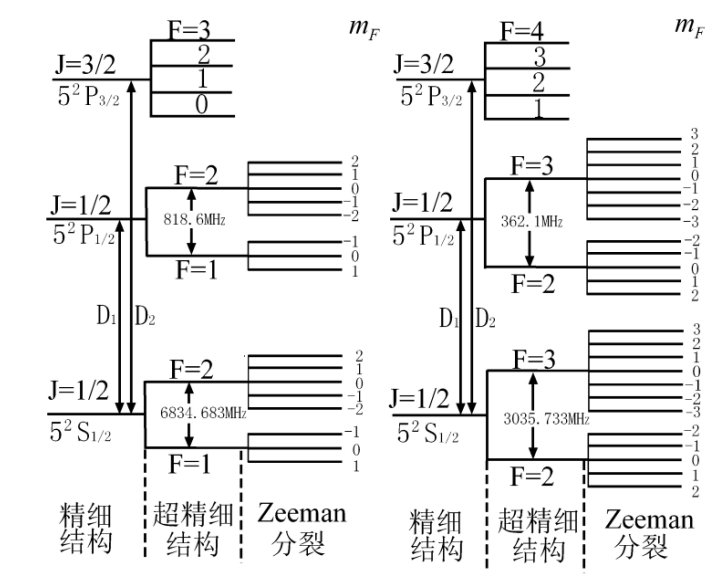
\includegraphics[width=0.8\textwidth]{能级图.png}
    \caption{铷原子能级结构图(能级之间的距离未按照比例画出)}
    \label{fig:energy_levels}
\end{figure}

在弱外磁场 $B_0$ 下，超精细结构能级将发生 Zeeman 劈裂，每个 $F$ 态分裂为 $(2F+1)$ 个 $m_F$ 子能级，其能量表达式为：
\[
E = E_0 + \frac{ah}{2}\left[ F(F+1) - I(I+1) - J(J+1) \right] + g_F m_F \mu_B B_0,
\]
其中 $a$ 为磁偶极常数，$\mu_B$ 为玻尔磁子。基于上述公式，相邻 Zeeman 子能级的能量间隔为：
\[
\Delta E_{m_F} = g_F \mu_B B_0.
\]

因此，在外磁场作用下，铷原子的基态能级呈现可分辨的 Zeeman 分裂结构，这为后续实现光抽运与磁共振提供了理论基础。

\subsubsection*{2.圆偏振光对 Rb 原子的激发与光抽运效应}
原子吸收光子的跃迁过程需满足能量守恒和角动量守恒。
对于角动量而言，光子的偏振状态决定其携带的角动量：
左旋圆偏振光（$\sigma^+$）具有 $+\hbar$ 的自旋角动量，右旋圆偏振光（$\sigma^-$）具有 $-\hbar$ 的角动量，
线偏振光则可视为 $\sigma^+$ 与 $\sigma^-$ 的叠加，总角动量为零。

在光与原子相互作用时，跃迁需满足如下选择定则：
\[
\Delta L = \pm 1, \quad \Delta F = 0, \pm 1, \quad \Delta m_F = \pm 1 \quad (\text{圆偏振光})
\]
以 $^{87}\mathrm{Rb}$ 的 D1 线激发（$5^2S_{1/2} \rightarrow 5^2P_{1/2}$）为例，若入射光为左旋圆偏振光 $\sigma^+$，则激发跃迁满足 $\Delta m_F = +1$。
因此，处于基态 $m_F$ 的原子将被选择性抽运至激发态 $m_F + 1$。由于激发态最高 $m_F$ 为 $+2$，而基态可达 $+2$，故最终大量原子将累积在无法再被激发的极限态 $m_F = +2$ 上，形成所谓的“暗态”。

然而，激发态粒子返回基态的过程（主要为自发辐射）在不同 $m_F$ 子能级之间的概率接近均匀。
因此，在经历多个抽运—退激循环后，原子在基态的分布将发生显著偏移，趋向于占据极端磁量子数状态。
这种偏离热平衡分布的现象称为\textbf{光抽运（optical pumping）}，其效果为将系统从等概率分布“泵送”至定向偏极化状态。

值得注意的是：
\begin{itemize}
  \item 右旋圆偏振光 $\sigma^-$ 会将原子抽运至 $m_F = -F$ 极端态；
  \item 线偏振光（$\pi$ 光）由于等价于 $\sigma^+ + \sigma^-$，不引起净抽运；
  \item 椭圆偏振光的抽运效应介于两者之间。
\end{itemize}

因此，只有当入射光为圆偏振状态（$\sigma^+$ 或 $\sigma^-$）且传播方向与外磁场方向一致时，才能实现明显的光抽运效应。该过程为实现磁共振信号探测提供了偏极化的前提条件。

\subsubsection*{3.弛豫过程}
光抽运过程将铷原子的基态粒子选择性地抽运至某一极端的磁量子数态（如 $m_F = +2$），从而形成远离热平衡的\textbf{偏极化分布}。
在没有其他干预下，系统会通过各种机制恢复至热平衡态，这一恢复过程称为\textbf{弛豫（relaxation）}。

在热平衡条件下，各个塞曼子能级上的粒子数 $N$ 服从玻尔兹曼分布：
\[
N = N_0 \exp\left(-\frac{E}{k_B T}\right)
\]
由于塞曼分裂能量在弱磁场下很小，热平衡下各 $m_F$ 态粒子数几乎相等。
但光抽运可使偏极化粒子数差异远超热分布，达到 $\sim 10^3$ 倍的量级，从而构造出对磁共振响应更强的非平衡态。

影响系统偏极化维持时间的主要弛豫机制包括：

\begin{enumerate}
  \item \textbf{原子与容器壁碰撞}：当 Rb 原子撞击玻璃泡壁时，其能量状态及自旋方向会显著扰动，导致极化迅速丧失。这是最主要的退极化来源。
  
  \item \textbf{原子间碰撞}：铷原子之间发生的自旋-自旋交换也会使粒子自旋随机化，尤其在高密度情况下更显著。
  
  \item \textbf{与缓冲气体的碰撞}：为延长偏极化寿命，实验中常充入氮气、氖气等缓冲气体。缓冲气体通过增加 Rb 原子的有效自由程、减少其与壁的直接碰撞，从而有效抑制退极化过程。由于缓冲气体自身磁性极弱，其与 Rb 原子的碰撞对磁子态扰动极小。
\end{enumerate}

温度变化也对弛豫过程具有显著影响：温度升高会导致 Rb 蒸气密度上升，增加原子间及与壁的碰撞频率，从而加快退极化；
反之，若温度过低，原子密度不足，将导致磁共振信号强度下降。
因此，实验中通常将样品泡温度控制在 $40^\circ\mathrm{C} \sim 60^\circ\mathrm{C}$ 范围内，以平衡偏极化维持与信号强度。

对于 $^{85}\mathrm{Rb}$，光抽运作用下的极端态为 $m_F = +3$，其弛豫过程与 $^{87}\mathrm{Rb}$ 类似。

综上所述，弛豫过程决定了偏极化的寿命和磁共振信号的锐度，是设计实验参数、优化信号获取的重要因素。

\subsubsection*{4.外磁场作用下塞曼子能级之间的磁共振}
通过光抽运过程，大量 $^{87}\mathrm{Rb}$ 或 $^{85}\mathrm{Rb}$ 原子被定向地抽运至基态的极端磁量子数态（如 $m_F = +2$ 或 $m_F = +3$），形成具有偏极化分布的非平衡体系。
在此基础上，若施加一个频率合适的交变磁场，将有可能诱导原子在塞曼子能级之间发生跃迁，即产生\textbf{磁共振现象}。

当样品处于一恒定的外磁场 $\mathbf{B}_0$ 中时，基态的每个超精细结构能级 $F$ 会发生塞曼劈裂，分裂为 $2F + 1$ 个子能级，其相邻能级之间的能量差为：
\[
\Delta E_{m_F} = g_F \mu_B B_0,
\]
其中 $g_F$ 为朗德因子，$\mu_B$ 为玻尔磁子。
若在垂直于 $\mathbf{B}_0$ 的方向上施加一个频率为 $\omega$ 的射频磁场 $\mathbf{B}_1$，则当满足如下\textbf{共振条件}时，将诱导共振跃迁发生：
\[
\hbar \omega = \Delta E_{m_F} = g_F \mu_B B_0.
\]

此时，处于极端态（如 $m_F = +2$）的粒子将吸收射频光子，跃迁至 $m_F = +1$ 等相邻态，破坏了原先的偏极化分布。
由于这些新跃迁态可以再次被光抽运激发，系统将建立一个新的动态平衡。

\textbf{磁共振的可观测性}体现在样品对光抽运光（$\sigma^+$）的吸收强度变化上：
\begin{itemize}
  \item 当未发生共振时，大多数原子处于暗态（如 $m_F = +2$），吸收光能力弱，透过光强大；
  \item 当满足共振条件时，粒子重新分布至多个 $m_F$ 态，对 $\sigma^+$ 光的吸收增强，透过光强下降；
\end{itemize}

因此，通过监测透过样品泡的光强随磁场或射频频率变化的响应，即可获取磁共振信号。
实验中通常固定射频频率 $\omega$，以扫场方式改变 $B_0$，在满足共振条件时观测到信号峰，进而求出朗德因子 $g_F$。

综上，磁共振过程本质上是原子吸收射频磁场能量导致的态跃迁行为，依赖于外磁场强度、射频频率及原子能级结构参数。该现象的观测为精确测定超精细结构与磁性参数提供了实验基础。

\subsubsection*{5.光探测}
在光泵磁共振实验中，入射至铷原子样品泡的 $\mathrm{D}_1$ 线圆偏振光（通常为 $\sigma^+$）不仅用于实现光抽运，同时也承担了磁共振信号的\textbf{探测功能}。具体而言，透过样品泡的光强包含了关于原子能级分布状态的信息，因而可以通过监测透光率的变化间接获取磁共振过程。

在无磁共振发生时，光抽运将大量原子抽运至基态极端态（如 $m_F = +2$），该态无法再被 $\sigma^+$ 光激发，导致系统对光的吸收减弱，即透过光强增强；当射频磁场 $\mathbf{B}_1$ 满足共振条件：
\[
\hbar \omega = g_F \mu_B B_0
\]
原子从 $m_F = +2$ 跃迁至 $m_F = +1$ 等其他子能级，这些子能级可以再次吸收光子，系统的光吸收增强，透光率下降。

因此，\textbf{共振信号的本质}是样品泡对光抽运光的吸收随外磁场或射频频率发生变化的表现。其具体特征包括：
\begin{itemize}
  \item 共振时，透过光强度出现下降；
  \item 非共振时，光抽运使系统恢复至暗态，透过光强回升；
  \item 该过程形成了可周期观测的光强调制信号，即磁共振曲线。
\end{itemize}

通过在实验中同步记录扫场信号与透过光强信号，可以得到磁共振发生时的共振点位置，从而反推出对应的 $B_0$ 值和 $g_F$ 值。

本实验中使用 $\mathrm{D}_1$ 线的 $\sigma^+$ 光一方面用于建立偏极化态，另一方面通过检测透过光强实现磁共振信号的高灵敏探测。相比直接测量微弱的射频能量吸收，\textbf{该光探测方法将射频信号“上转换”为可见光强度变化，从而显著提高了信号探测灵敏度，达 $10^7 \sim 10^8$ 倍}，是该实验的重要技术优势。

\subsection*{【实验仪器】}
\begin{table}[h!]
	\centering
	\begin{tabular}{|p{5cm} p{4cm} p{5cm}|}
		\hline
		仪器名称 & 型号 & 参数 \\
		\hline\hline
		函数发生器 & AFG-2225 & - \\
		
		光磁共振实验装置电源 & DH870A & - \\
		
		示波器 & RIGOL ~ DS4022 & 2通道 200 MHz \\
		\hline		
	\end{tabular}
	\caption{实验仪器及参数}
	\label{tab:instruments}
\end{table}
    实验中我们还需要计算亥姆霍兹线圈能够产生的磁场大小，这就需要我们从仪器上读出亥姆霍兹线圈的有关参数。
\begin{table}[h!]
    \centering
    \caption{亥姆霍兹线圈的参数}
    \begin{tabular}{|c|c|c|c|}
        \hline
         - & 水平场线圈 & 扫场线圈 & 垂直场线圈 \\
        \hline
        线圈匝数 & 250 & 250 & 100 \\
        \hline
        有效半径 & 0.2399$\,\mathrm{m}$ & 0.2420$\,\mathrm{m}$ & 0.1530$\,\mathrm{m}$ \\
        \hline
    \end{tabular}
\end{table}

同时我们知道亥姆霍兹中心磁场大小和电流的关系公式
\[
H = \frac{16\pi}{5^{3/2}} \cdot \frac{N}{r} \cdot I \cdot 10^{-3} \left(\mathrm{Gs}\right)
\]
其中，$N$是线圈匝数，$I$是电流，$r$是线圈半径。

\subsection*{【实验内容】}
\begin{enumerate}
	\item 确认光路上各元件共轴并与地磁水平分量平行（或反平行）。
	\item 预热约15分钟。辅助电源的池温和灯温指示亮时，即可进行实验观测。
	\item 观察方波扫场的光抽运现象，理解光抽运的物理过程及光抽运信号检测技术方法。
	重点：分析产生光抽运的实验条件。

	\item 观察垂直磁场和水平磁场对方波扫场光抽运信号影响，记录、分析不同磁场方向和强度的实验结果；调节垂直磁场（方向和强度）使抽运信号达最大。
	\item 仔细观察三角波扫场的光抽运现象，记录不同磁场强度和方向对光抽运信号的影响。
	通过与方波扫场的实验结果进行比较，分析所观察到的抽运现象，从而进一步理解产生光抽运的实验条件。

	\item 观测共振吸收，分析85Rb和87Rb的 gF因子：
	\begin{itemize}
		\item 设定简谐射频场频率（可选600 ～ 800 kHz），调节适量的输出幅值； 

		\item 缓慢增加水平场强度，观察记录抽运信号和共振信号的变化，区分两种信号物理过程，找出共振吸收实验条件；
		\item 随着水平场强度的缓慢增加，观察记录同位素共振信号的变化； 
		\item 采用反向平均消除地磁或抽运信号定位方法，观测85Rb和87Rb共振吸收； 
		\item 测量一组不同简谐频率（400kHz ~ 1MHz 之间）射频场作用的85Rb和87Rb共振吸收数据，采用曲线拟合方法分别分析85Rb和87Rb 的gF实验结果。
	\end{itemize}

	\item 实验完毕
	\begin{itemize}
		\item 将仪器各旋扭复位并切断电源；
		\item 将仪器和实验资料摆放整齐；
		\item 清洁桌面，不要遗留个人用品。经任课老师确认并在《近代物理实验室仪器设备使用登记表》上签字方可离开实验室。
	\end{itemize}
\end{enumerate}

\subsection*{【实验过程和数据处分析处理】}
仔细阅读上述实验过程，并检查实验仪器完整可用之后我们开始实验。
这里的主要实验装置都已经调节好并放置在遮光罩内部，我们稍微掀起遮光罩的一侧检查装置是否完整。
在这个过程中我们特别需要借助指南针检查装置放置的方向是否和地磁场平行。

\begin{figure}[h!]
    \centering
    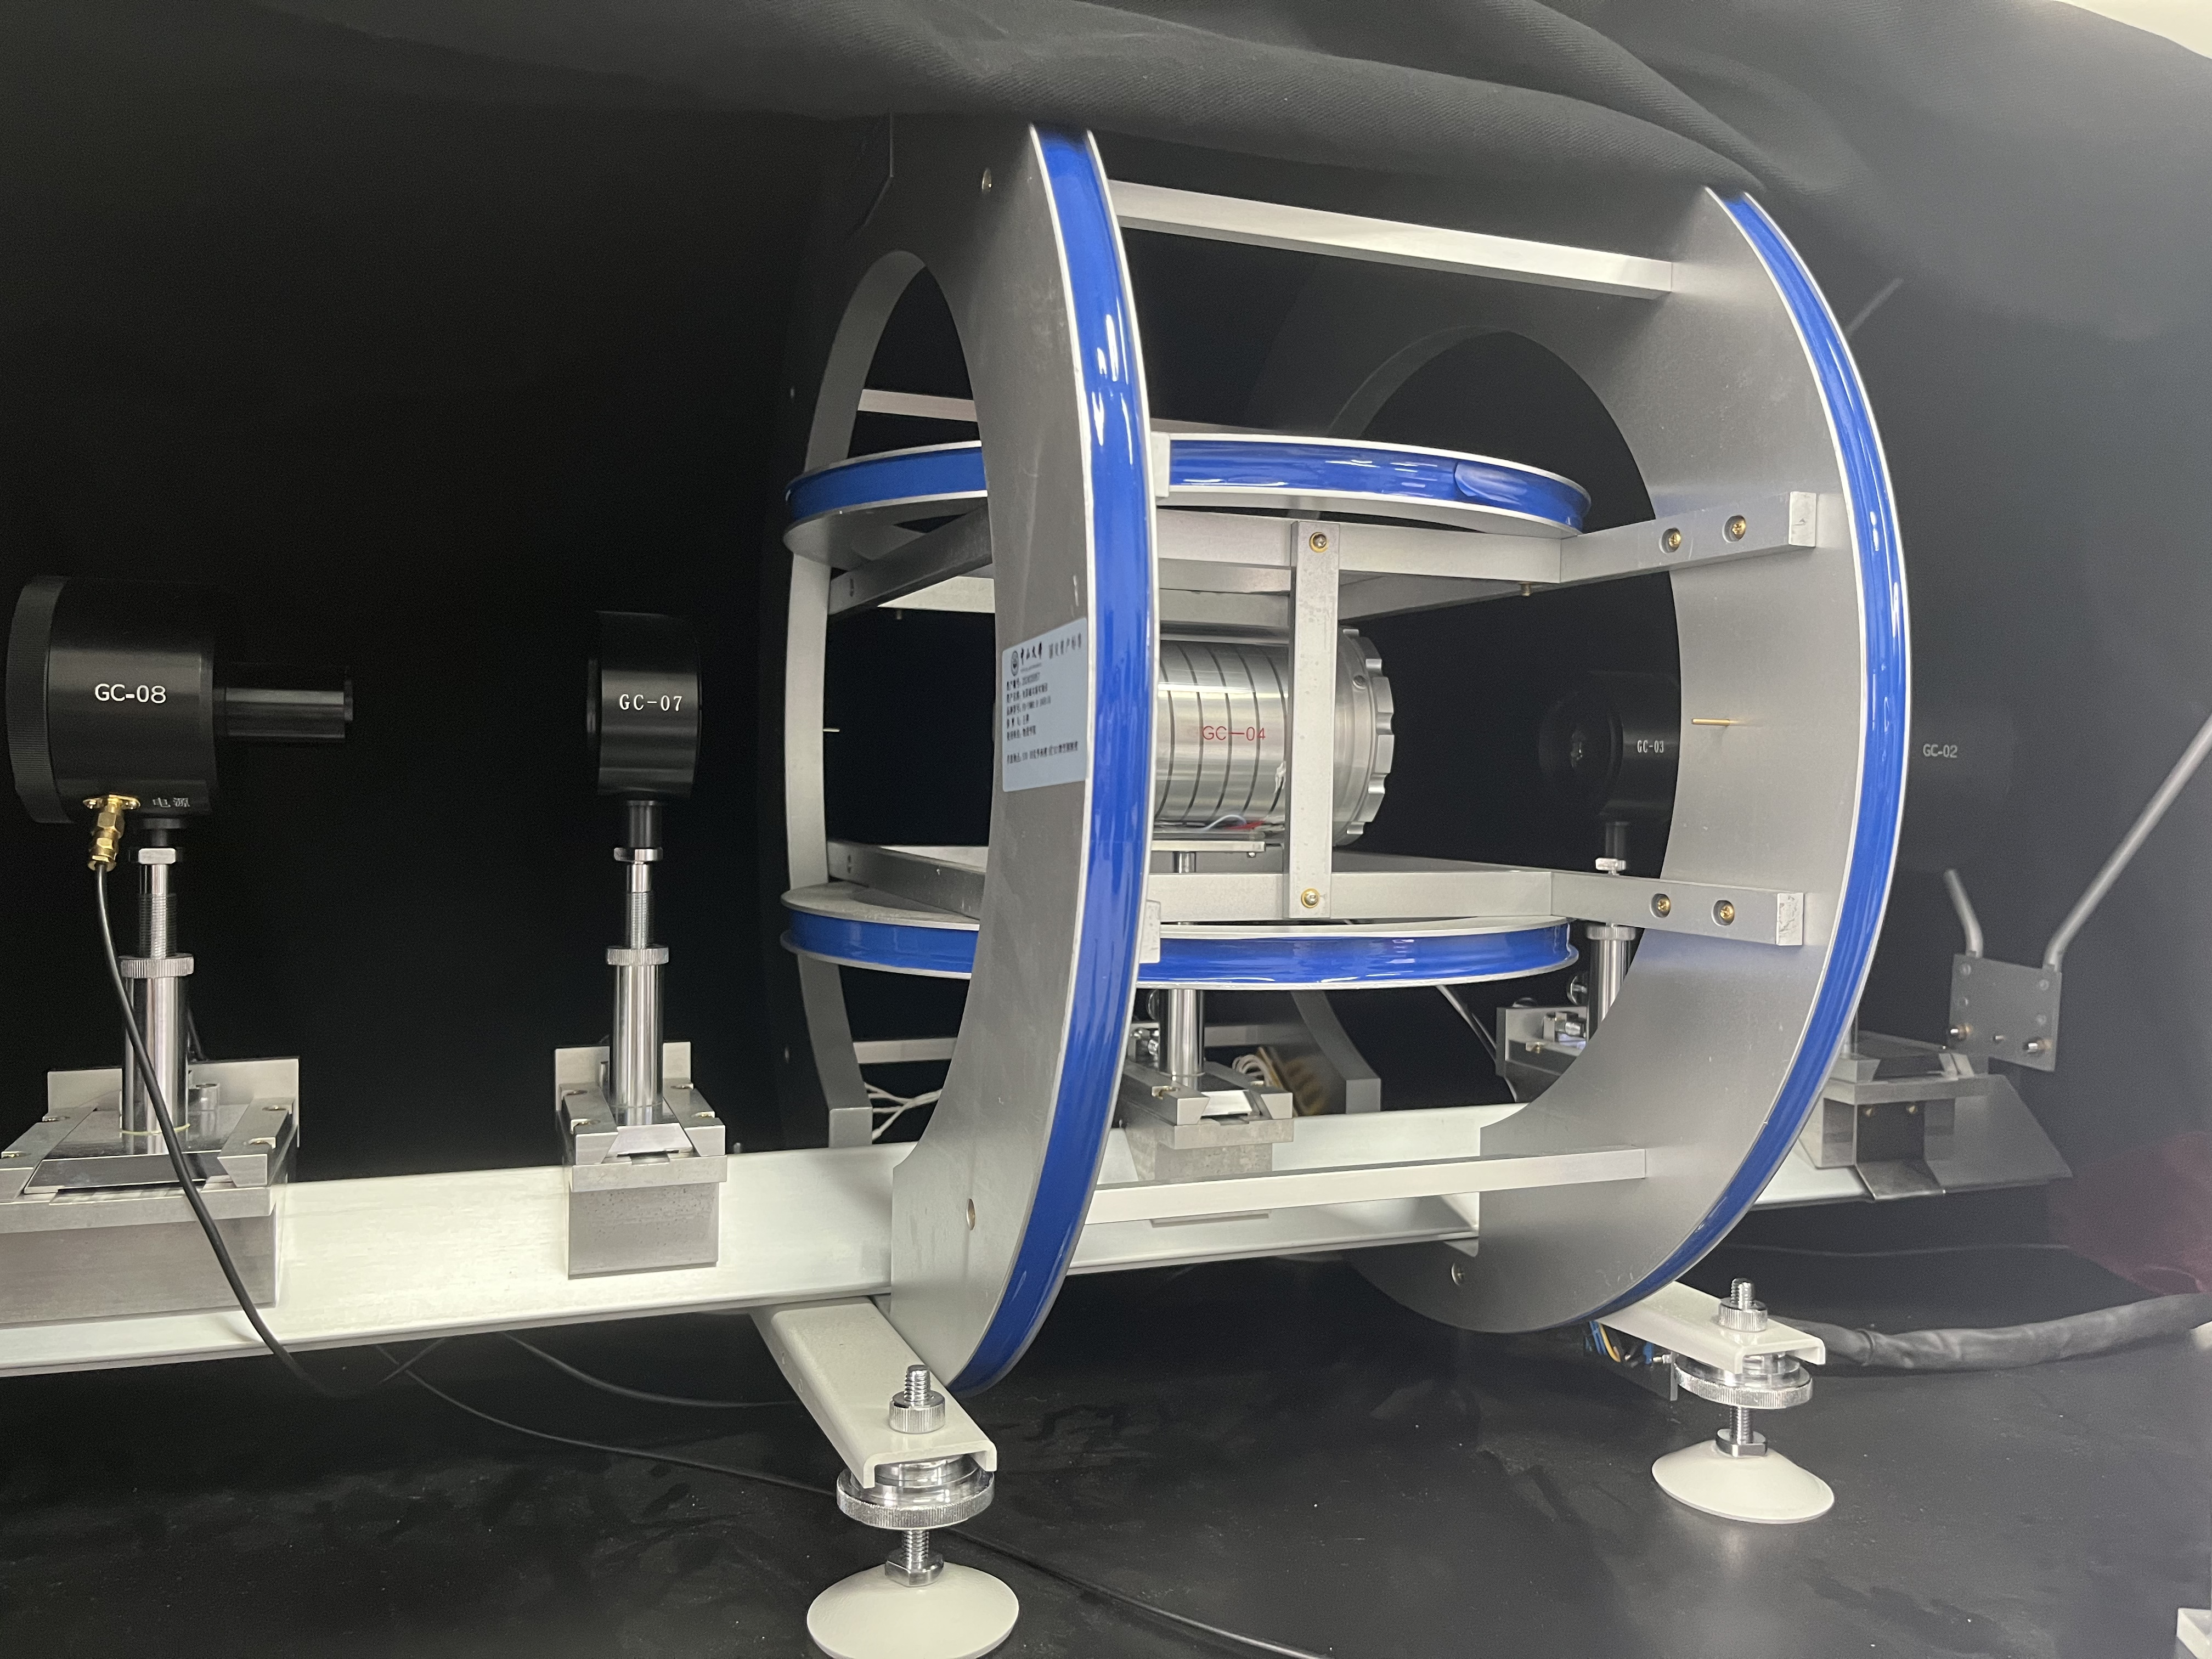
\includegraphics[width=0.65\textwidth]{装置检查.jpg}
    \caption{实验装置检查}
    \label{fig:device_check}
\end{figure}

确认装置完整之后，我们盖上遮光罩，开启电源开关，预热大约15分钟。
看到辅助电源的池温和灯温指示亮时，表示预热成功，即可进行实验观测。

\subsubsection*{1.观察方波和三角波扫场的光抽运现象}
先调节水平磁场和垂直磁场到合适位置，再在此基础上施加扫描磁场。
我们首先施加的是方波形式的扫描磁场，适当调节扫场幅度便能看到光抽运现象。

此时我们再调节垂直场和水平场的大小，使得观察到光抽运信号达到最大，如\ref{fig:方波抽运现象}所示。

\begin{figure}[h!]
    \centering
    \includegraphics[width=0.65\textwidth]{方波抽运19_58.png}
    \caption{方波扫场时光抽运现象}
    \label{fig:方波抽运现象}
\end{figure}

此时的水平场电流是$0.019\mathrm{A}$，垂直场电流是$0.058\mathrm{A}$。
对应换算之后可以得到水平场和垂直场的磁场大小分别为$0.0890\mathrm{Gs}$和$0.1704\mathrm{Gs}$。

对于三角波扫场也是类似的操作，我们最后得到的实验现象如\ref{fig:三角波抽运现象}所示。

\begin{figure}[h!]
    \centering
    \includegraphics[width=0.65\textwidth]{三角抽运19_58.png}
    \caption{三角波扫场时光抽运现象}
    \label{fig:三角波抽运现象}
\end{figure}

此时的水平场电流是$0.019\mathrm{A}$，垂直场电流是$0.058\mathrm{A}$。
对应换算之后可以得到水平场和垂直场的磁场大小分别为$0.0890\mathrm{Gs}$和$0.1704\mathrm{Gs}$。

此处由于方波和三角波的扫场振幅相同，因此我们观察到出现光抽运现象的磁场强度也十分相近。

\subsubsection*{2.测量磁共振并计算g因子} 
\paragraph{观测共振信号}
按照上述的实验步骤，我们设置好简谐射频场的频率，适当调节其输出幅值，在这里我们采用的输出幅值是$7.5\mathrm{V}$。
此时的扫场波形设置为三角波，能够观察到共振现象。
这里值得注意的是，为了在实验中方便地区分光抽运信号和共振信号，我们可以在观察到信号之后，关掉射频场的输出。
如果示波器上的信号随着射频场的关闭而消失，则说明该信号是共振信号；若信号不消失，则说明该信号是光抽运信号。

在这个实验中为了抵消地磁场的垂直分量，我们设置垂直场电流为$0.058\mathrm{A}$，对应的磁场大小为$0.1704\mathrm{Gs}$。

接着我们开始测量共振信号，在这个过程中我们主要调节水平场电流，记录共振信号的最低点和三角波的最低点重合时对应的磁场大小数据。
部分测量图像如图\ref{fig:共振信号1}和\ref{fig:共振信号2}所示
\begin{figure}[h!]
    \centering
    \begin{minipage}{0.48\textwidth}
        \centering
        \includegraphics[width=\textwidth]{共振324_58.png}
        \caption{共振信号1}
        \label{fig:共振信号1}
    \end{minipage}
    \hfill
    \begin{minipage}{0.48\textwidth}
        \centering
        \includegraphics[width=\textwidth]{共振327_58.png}
        \caption{共振信号2}
        \label{fig:共振信号2}
    \end{minipage}
\end{figure}

其中图\ref{fig:共振信号2}，并不是我们想要观测的共振信号，但是图中的现象是在水平磁场接近共振点时才会出现的现象，即在一个扫描周期中出现多个峰。
这种现象可以辅助我们判断此时出现的是共振信号还是光抽运信号。

最后我们测量了在射频场频率在$300\mathrm{kHz}$到$800\mathrm{kHz}$之间时，共振信号的变化。
结果如图\ref{fig:共振图}所示

\begin{figure}[h!]
    \centering
    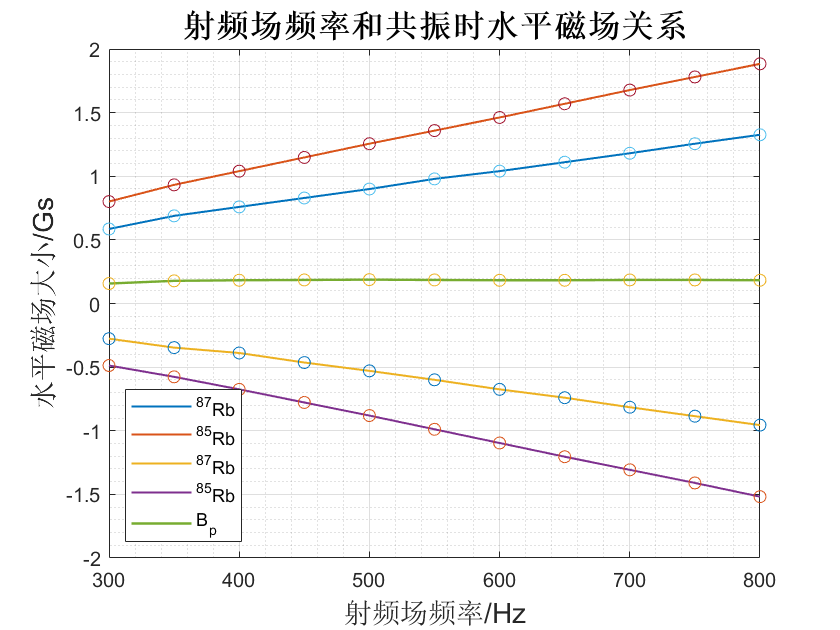
\includegraphics[width=0.8\textwidth]{共振图.png}
    \caption{共振图}
    \label{fig:共振图}
\end{figure}

\paragraph{计算g因子}

接下来我们使用拟合的方式计算两种Rb的g因子拟合效果的参数如下图所示

\begin{figure}[h!]
    \centering
    \begin{minipage}{0.48\textwidth}
        \centering
        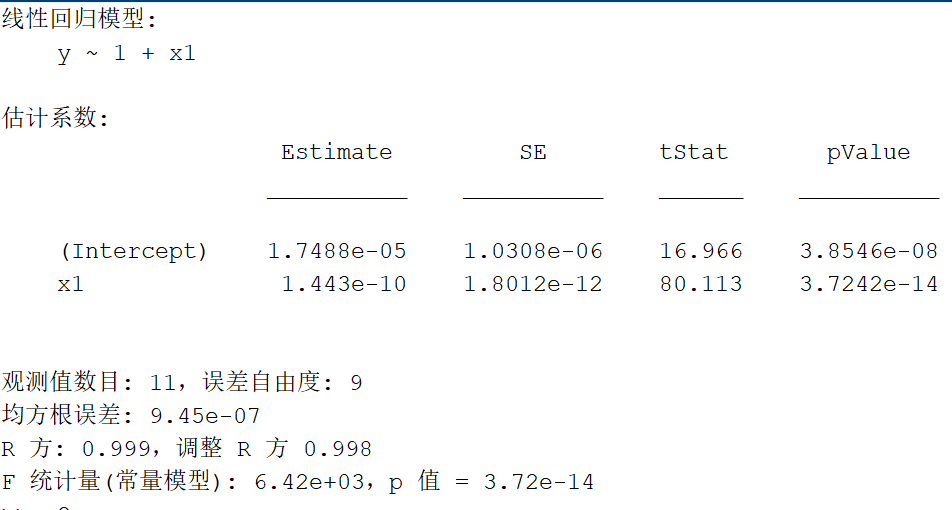
\includegraphics[width=\textwidth]{p1.png}
        \caption{拟合图1}
        \label{fig:拟合图1}
    \end{minipage}
    \hfill
    \begin{minipage}{0.48\textwidth}
        \centering
        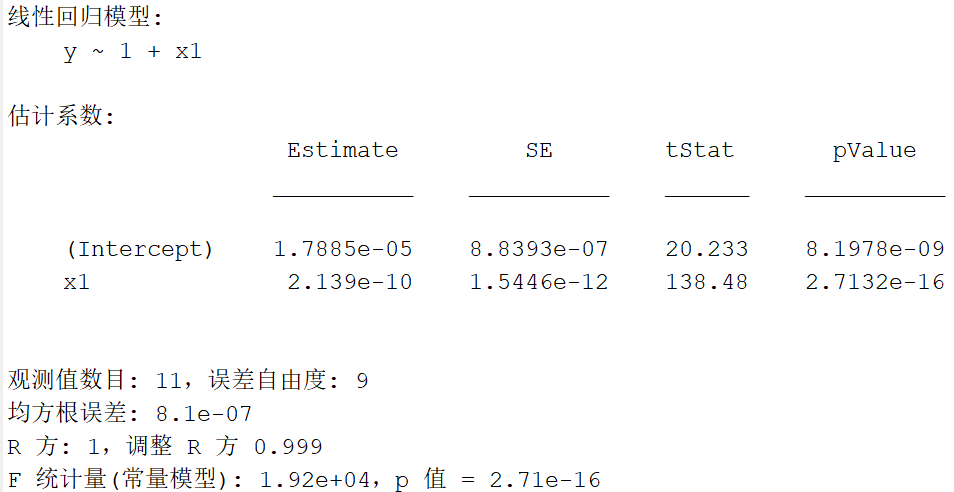
\includegraphics[width=\textwidth]{p2.png}
        \caption{拟合图2}
        \label{fig:拟合图2}
    \end{minipage}
    
    \vspace{0.5cm}
    
    \begin{minipage}{0.48\textwidth}
        \centering
        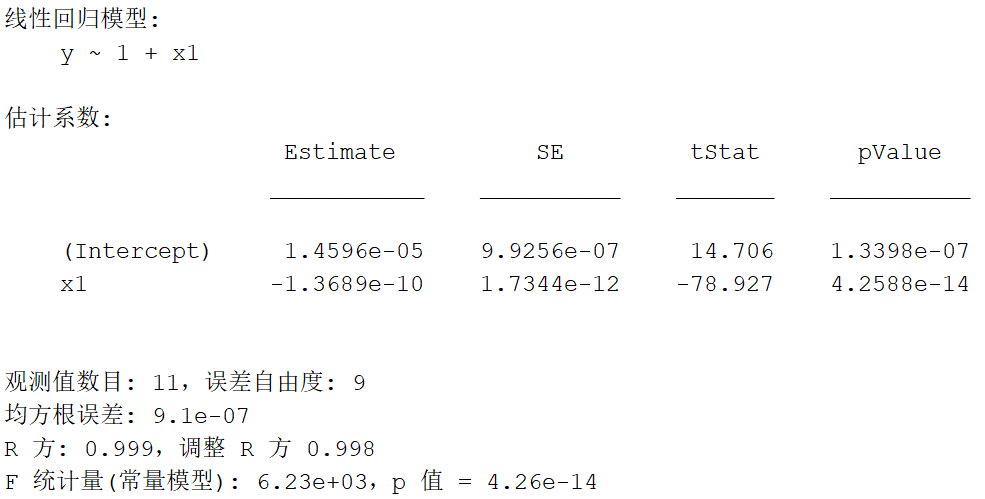
\includegraphics[width=\textwidth]{p3.png}
        \caption{拟合图3}
        \label{fig:拟合图3}
    \end{minipage}
    \hfill
    \begin{minipage}{0.48\textwidth}
        \centering
        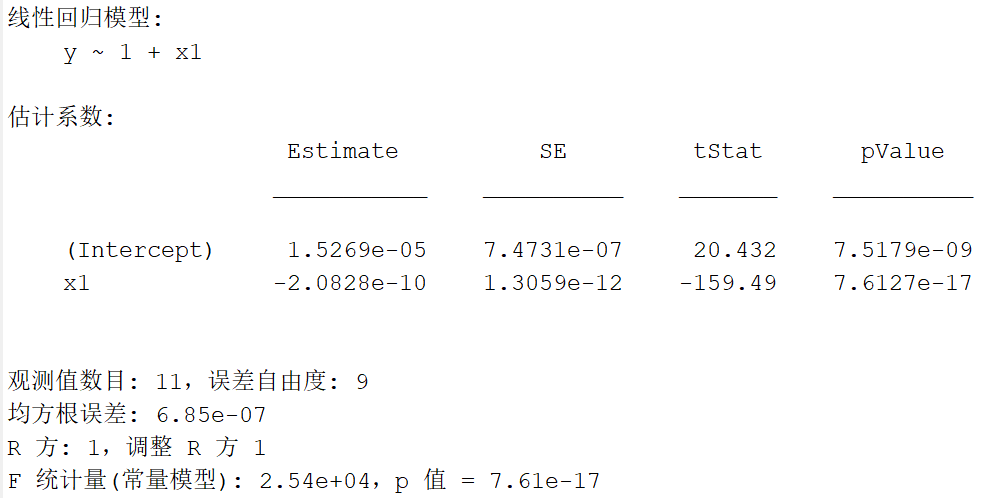
\includegraphics[width=\textwidth]{p4.png}
        \caption{拟合图4}
        \label{fig:拟合图4}
    \end{minipage}
    \caption{Rb的g因子拟合结果}
    \label{fig:拟合结果}
\end{figure}

可见四组数据的拟合R放都达到了$0.999$以上，说明拟合效果很好，我们可以用拟合得到的数据继续计算g因子。

给出g因子计算公式如下
\[
g = \frac{h}{\mu_{B\, k}}
\]
其中$h$是普朗克常数，$\mu_{B}$是玻尔磁子，$k$是拟合得到的斜率。

最后计算得到的g因子结果如下
\begin{table}[h!]
    \centering
    \begin{tabular}{|c|c|}
        \hline
        $^{85}\mathrm{Rb}$ & $ 0.34 \pm 0.01$ \\
        \hline
        $^{87}\mathrm{Rb}$ & $ 0.50 \pm 0.01$\\
        \hline
    \end{tabular}
    \caption{计算得到的g因子结果}
    \label{tab:g因子结果}
\end{table}

\paragraph{误差分析}

根据参考文献，$^{85}\mathrm{Rb}$和$^{87}\mathrm{Rb}$的g因子理论值分别为$1/3 \approx 0.333$和$1/2 = 0.5$。
对比我们实验测得的结果：$^{85}\mathrm{Rb}$的g因子为$0.34 \pm 0.01$，$^{87}\mathrm{Rb}$的g因子为$0.50 \pm 0.01$，可以看出实验结果与理论值基本吻合，在误差范围内。
而主要的不足在测量精度上，

总体而言，本实验测得的g因子与理论值非常接近，证明了实验方法的可靠性和有效性。

\subsection*{【思考题】}
\begin{enumerate}
  \item \textbf{在消除地磁场的垂直分量影响时，方波信号应该满足什么条件才能观察到抽运信号？为什么？}

  要观察到光抽运信号，方波磁场必须使总磁场（包括地磁场分量和方波叠加场）在一个周期内经过零点。也就是说，方波磁场的幅值 $B_m$ 应大于地磁场在水平方向或垂直方向上的分量，以确保总磁场可以由正值跳变为负值，从而实现塞曼能级简并和重新分裂的全过程。

  当方波磁场改变符号经过零点时，原本偏极化的原子失去极化（能级简并），再重新建立抽运态，从而在一个周期内形成透光率的明显变化，产生可观测的抽运信号。\cite{wu1999modernexp,zheng1988modernexp,he2003modernexp,wu1999scienceexp,lin1999tutorial}

  \vspace{0.5em}

  \item \textbf{为什么 D2 线的存在会使系统无法实现偏极化？在实验中通常会出现纯抽运信号和磁共振信号，这两种信号分别是怎样产生的？采取什么样的实验手段可以区分它们？}

  D2 线对应的是 $5^2S_{1/2} \rightarrow 5^2P_{3/2}$ 跃迁。该激发态由于 $J = 3/2$，拥有更多的磁子能级，其退激过程不能有效地将粒子导向某一特定的极端态，因此无法建立明显的偏极化态，导致光抽运效率低。

  \textbf{纯抽运信号}：在仅有光抽运、无射频场作用的情况下，粒子逐步积累至暗态，透过光强度随时间逐渐增强，构成周期性的抽运信号。

  \textbf{磁共振信号}：在施加射频磁场后，满足共振条件的塞曼能级间发生跃迁，打破偏极化，透过光强周期性减弱，从而形成附加于抽运信号之上的共振结构。

  \textbf{区分方法}：关闭射频信号源时只存在抽运信号；开启射频场并调整至共振频率时，信号上会出现明显的共振峰或谷。对比两者，即可区分纯抽运与磁共振信号。

  \vspace{0.5em}

  \item \textbf{在调节水平扫描磁场的幅度时，如何判断其大小是否合适？当水平磁场和水平扫描取不同方向时，总磁场的大小和方向如何确定？}

  合理的扫描磁场幅度应能覆盖磁共振所需的 $B_0$ 范围。若幅度过小，无法扫描至共振点，将无法观测到磁共振信号；若过大，可能导致信号过宽、灵敏度下降。因此，可通过调整扫描幅度使得共振信号出现在扫描周期的中间区域，且具有良好的信噪比作为判断标准。

  当恒定水平磁场 $B_0$ 与扫描磁场 $B_m(t)$ 不同向（如一为正方向、一为负方向）时，总磁场为两者矢量叠加：
  \[
  B_{\text{tot}}(t) = B_0 + B_m(t)
  \]
  扫描过程中，总磁场将随时间变化从某一方向逐步增大或减小，从而可能在某一时刻满足磁共振条件。应根据方向关系合理设置初始恒定场与扫描场的相对极性，以保证总磁场在一个周期内穿越共振点。
\end{enumerate}


\bibliography{ref.bib} %biblatex -> 'xelatex->pdfletax->xelatex'
\bibliographystyle{ieeetr}

\subsection*{【原始数据的记录】}
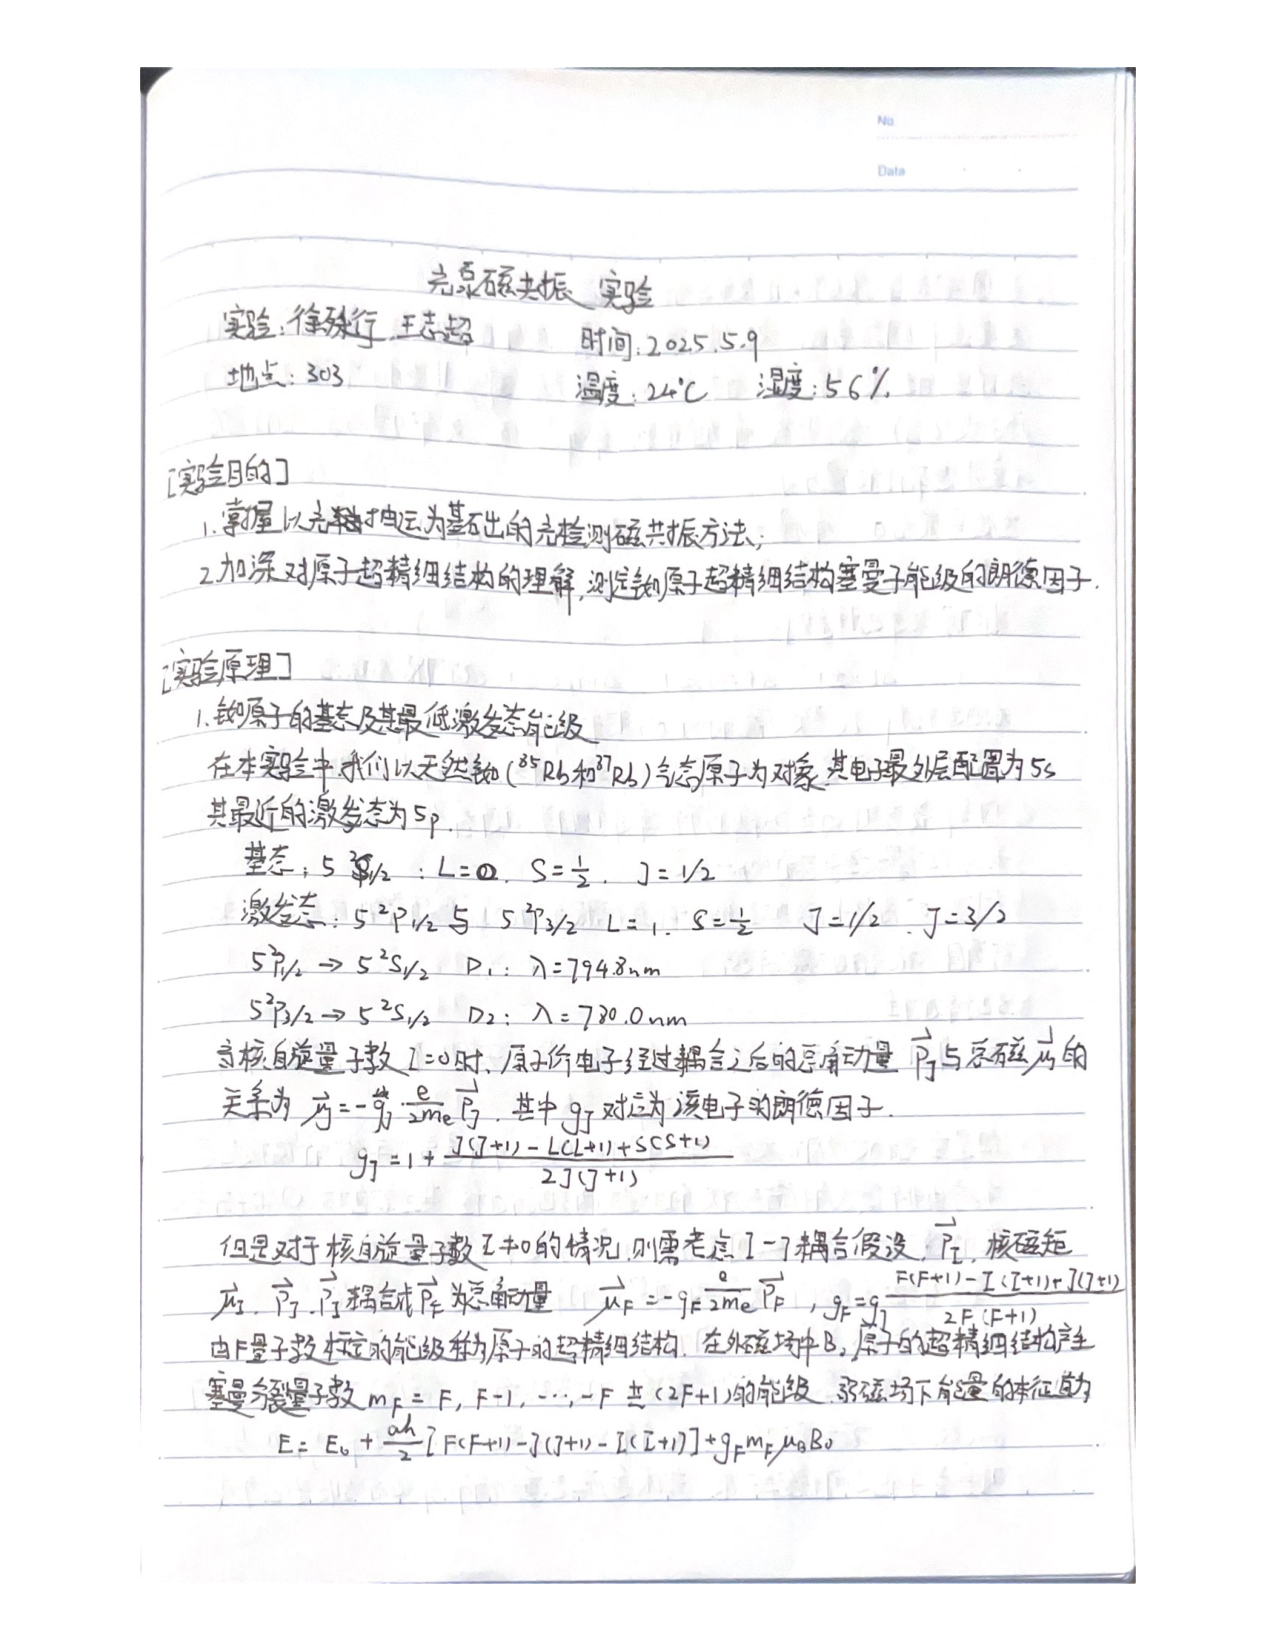
\includepdf[pages=-]{光泵磁共振scan.pdf}

\end{document}

